\lstset{language=Alloy}.



\section{Alloy Model}
In this section we show the model of the system, by formalizing it with Alloy. This step is strictly important, due to its consistency. 
In particular it describes the basic structure and the behavior of our system based on FOL.
In our alloy model we will show a typical day in the market. \\
We will describe the main objects involved as signature, with relative constraints, trying to reach a compromise between readability and complexity.
\par
We will exclude from the model some classes, and some tests, because they are useless to describe the model.
For example, we will exclude:
\begin{itemize}
\item the \textit{Elderly people} that are not involved with Reservation/Visit and therefore they will enter directly in the market in certain time slots;
\item the \textit{Receptionist} that acts as intermediary between Mobile User and the system. 
\item \textit{Market maximum capacity test}: even if this is one of most important goal to reach, we could not describe it in a sufficient way.
\end{itemize}
\pagebreak
In the following model, we discuss the possible choices that the users can do, such as booking a Reservation/Visit, and the constraints imposed by their choices.
In particular we describe:
\begin{itemize}
\item \textit{Reservation and its insertion} on the Queue with the number assigned to it;
\item \textit{Visit booking} between the time slots entered by the users and the shopping time based on its size choosen.
\end{itemize}
\par
An other important aspect it's the formalization of the QRCode. Users enters in the market with a QRCode if and only if it's valid but not submitted yet. Otherwise, with different boolean values the QRCode signature could have different meaning. All possibile type of QRCode could be:
\begin{itemize}
    \item \textit{Valid and not submitted}: QRCode owner has booked an appointment (either a Reservation or a Visit) and he hasn't entered yet;
    \item \textit{Submitted and valid}: the QRCode owner is in the market ;
    \item \textit{Submitted and not valid}: the QRCode is already used by the owner;
\end{itemize}


The model is organized temporaly in time slots of 30 minutes each. This way make easier the Visit schedule. The time estimation of each appointment is determined by the bag size. In particular it could be:
\begin{itemize}
\item \textit{Small}: it occupies 1 slot in the schedule, that is 30 minutes;
\item \textit{Medium}: it occupies 2 slots in the schedule, that is 60 minutes;
\item \textit{Large}: it occupies 3 slots in the schedule, that is 90 minutes;
\end{itemize}


In the following model, we describe the situation in which one reservation is booked and consequently inserted in the queue. (figure 4.6)

In particular we will list 2 queue:
\begin{itemize}
\item Q is the queue before the insertion.
\item Q2 is the queue after the insertion.
\end{itemize}



Instead, in the figure~\ref{deInQueue} describes the situation in which one reservation is deleted from the queue.
This means that the reservation will be removed by its user.
We prefer not to update the reservation number, because it implies to duplicate all reservation in the queue behind the one that was cancelled. This could involve less readability.

\pagebreak

\lstinputlisting[language=alloy]{model/alloy.als}

\pagebreak

\begin{figure}[H]
  \label{marketOpened}
  \centering
  \makebox[\linewidth]{
  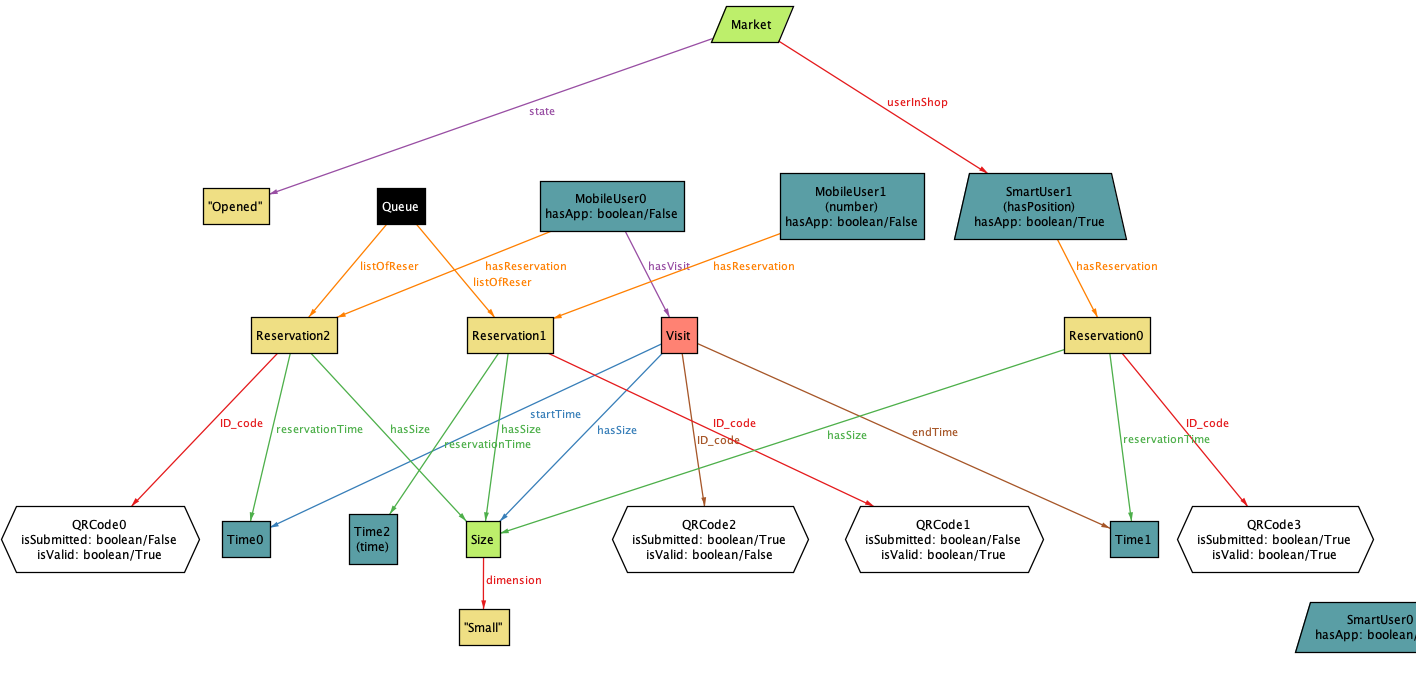
\includegraphics[scale=0.40]{report_alloy/marketOpened.png}}
    \caption{Rapresentation of the market opened in a generic day.}
\end{figure}

\begin{figure}[H]
  \label{marketClosed}
  \centering
  \makebox[\linewidth]{
  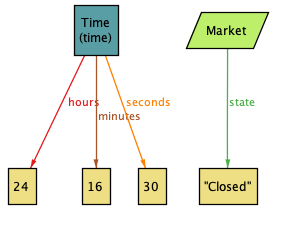
\includegraphics[scale=0.52]{report_alloy/marketClosed.png}}
    \caption{The market is closed. In this case, there aren't any users in the market.}
\end{figure}

\begin{figure}[H]
  \label{shorReserv}
  \caption{Rapresentation of the market opened in a generic day. This is the result of the showReservation predicate that focuses on Reservaitons.}
  \centering
  \makebox[\linewidth]{
  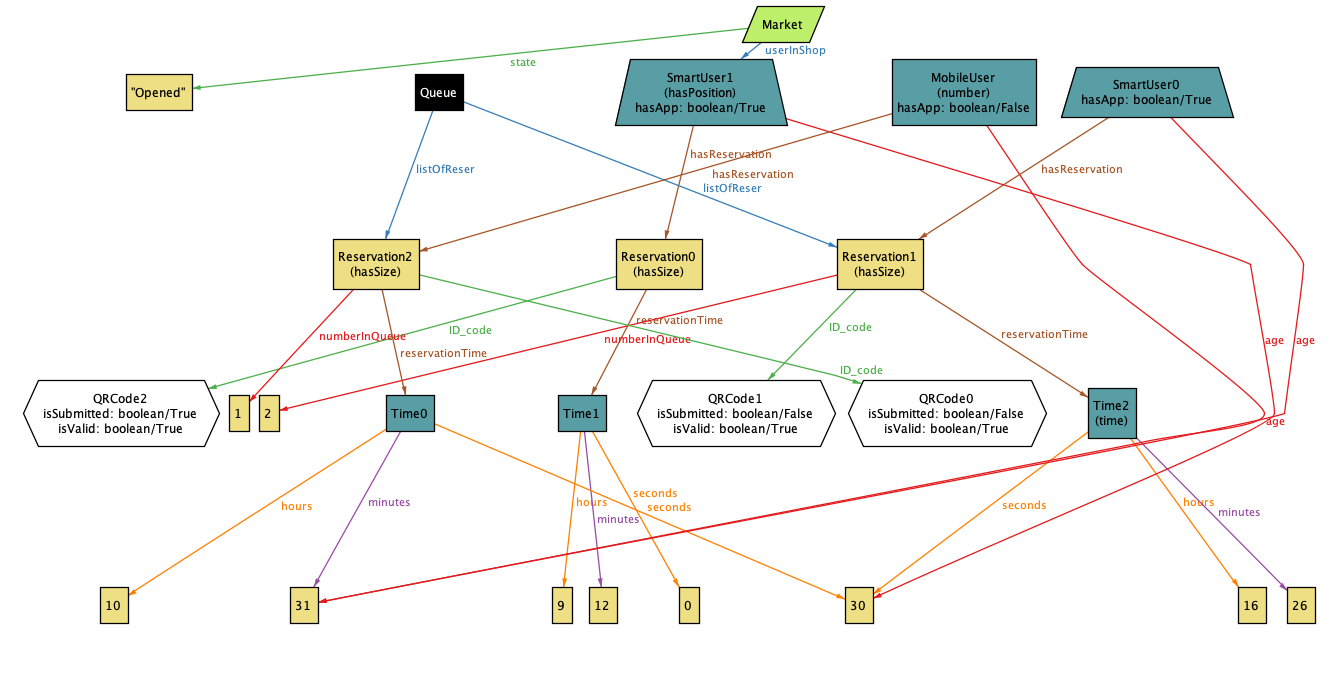
\includegraphics[scale=0.42]{report_alloy/shorReserv.png}}
    
\end{figure}

\begin{figure}[H]
\caption{Rapresentation of the market opened in a generic day. This is the result of the showVisit predicate that focuses on Visits.}
  \label{showVisit}
  \centering
  \makebox[\linewidth]{
  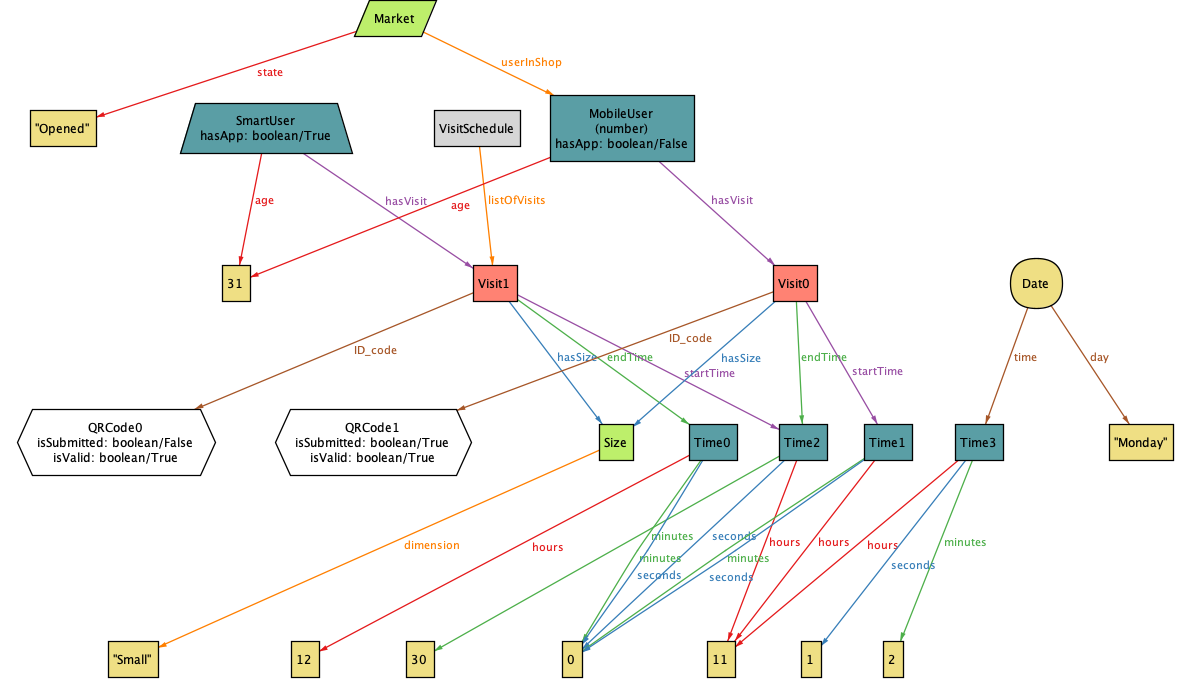
\includegraphics[scale=0.45]{report_alloy/showVisit.png}}
    
\end{figure}


\begin{figure}[H]
  \label{addInQueue}
  \centering
  \makebox[\linewidth]{
  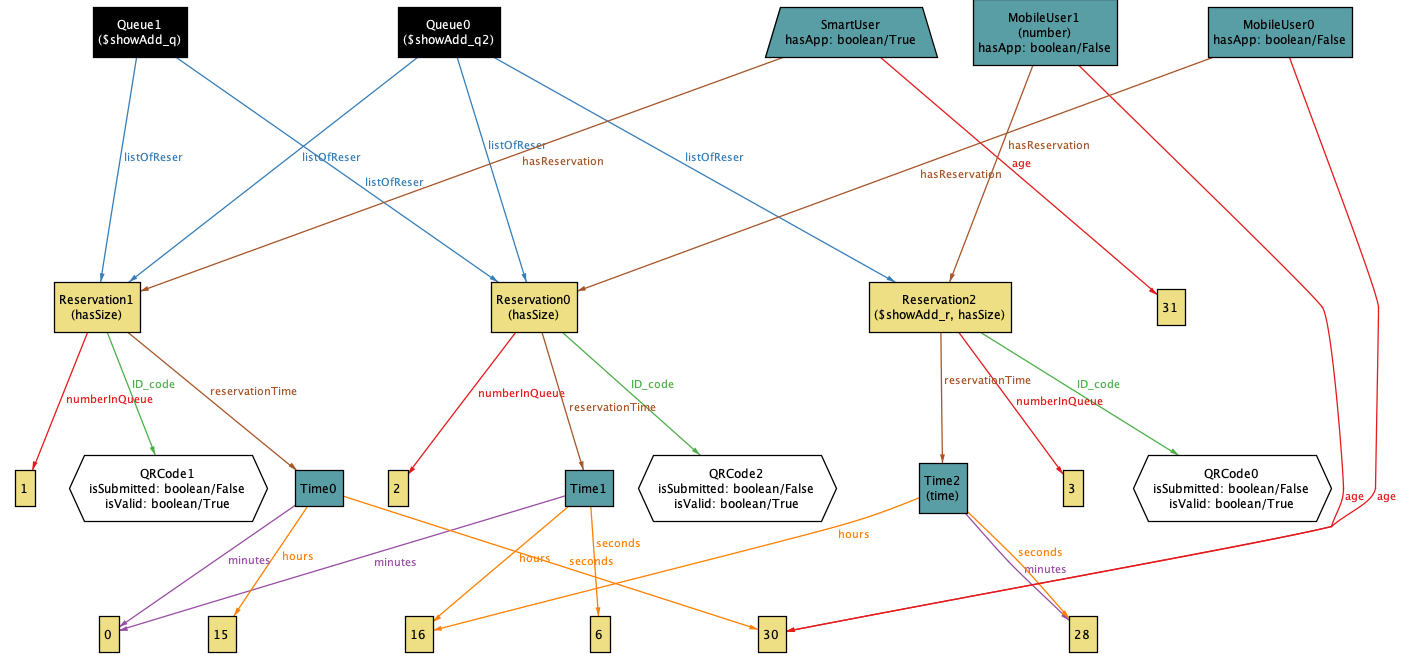
\includegraphics[scale=0.42]{report_alloy/addInQueue.png}}
    \caption{Queue insert reservation}
\end{figure}


\begin{figure}[H]
  \label{deInQueue}
  \centering
  \makebox[\linewidth]{
  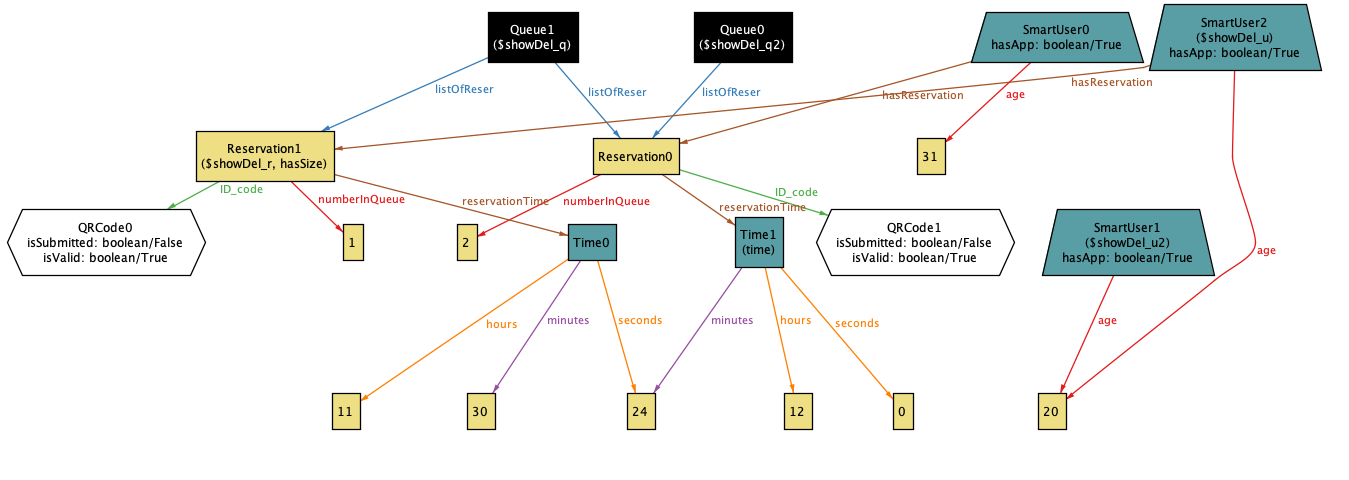
\includegraphics[scale=0.45]{report_alloy/deInQueue.png}}
    \caption{Queue remove reservation}
\end{figure}

\section{Alloy Results}

\begin{figure}[H]
  \label{pred1}
  \centering
  \makebox[\linewidth]{
  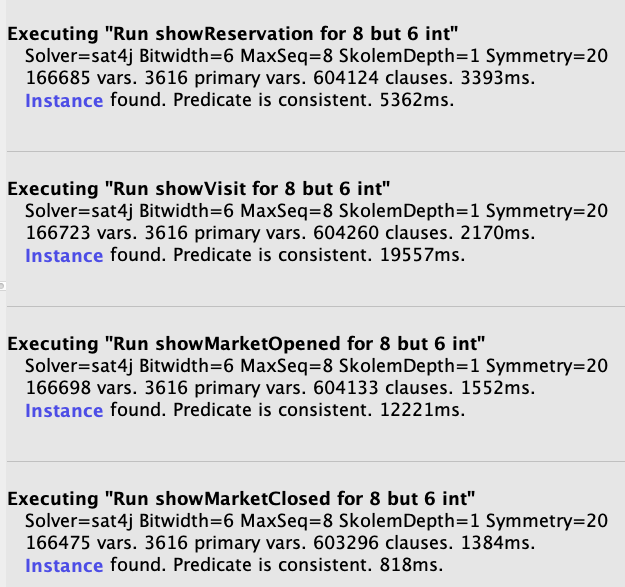
\includegraphics[scale=0.35]{report_alloy/pred1.png}}
    \caption{Results of the predicates}
\end{figure}

\begin{figure}[H]
  \label{reportAssert}
  \centering
  \makebox[\linewidth]{
  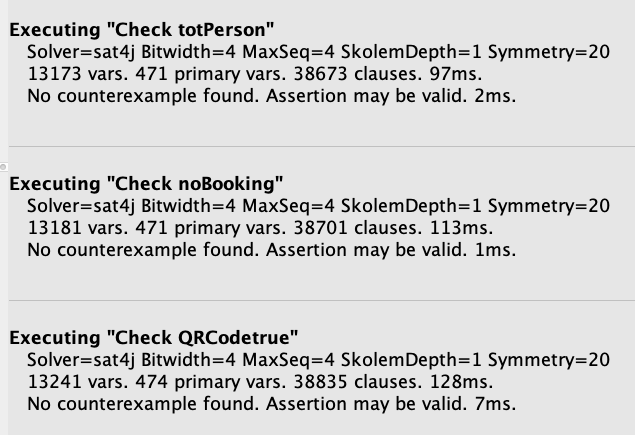
\includegraphics[scale=0.35]{report_alloy/reportAssert.png}}
    \caption{Results of the assers}
\end{figure}